\iffalse
This file is protected by Copyright. Please refer to the COPYRIGHT file
distributed with this source distribution.

This file is part of OpenCPI <http://www.opencpi.org>

OpenCPI is free software: you can redistribute it and/or modify it under the
terms of the GNU Lesser General Public License as published by the Free Software
Foundation, either version 3 of the License, or (at your option) any later
version.

OpenCPI is distributed in the hope that it will be useful, but WITHOUT ANY
WARRANTY; without even the implied warranty of MERCHANTABILITY or FITNESS FOR A
PARTICULAR PURPOSE. See the GNU Lesser General Public License for more details.

You should have received a copy of the GNU Lesser General Public License along
with this program. If not, see <http://www.gnu.org/licenses/>.
\fi
%----------------------------------------------------------------------------------------
% Update the docTitle and docVersion per document
%----------------------------------------------------------------------------------------
\def\docTitle{OpenCPI Overview}
\def\docVersion{1.4}
%----------------------------------------------------------------------------------------
\documentclass{article}
\iffalse
This file is protected by Copyright. Please refer to the COPYRIGHT file
distributed with this source distribution.

This file is part of OpenCPI <http://www.opencpi.org>

OpenCPI is free software: you can redistribute it and/or modify it under the
terms of the GNU Lesser General Public License as published by the Free Software
Foundation, either version 3 of the License, or (at your option) any later
version.

OpenCPI is distributed in the hope that it will be useful, but WITHOUT ANY
WARRANTY; without even the implied warranty of MERCHANTABILITY or FITNESS FOR A
PARTICULAR PURPOSE. See the GNU Lesser General Public License for more details.

You should have received a copy of the GNU Lesser General Public License along
with this program. If not, see <http://www.gnu.org/licenses/>.
\fi
\author{} % Force author to be blank
%----------------------------------------------------------------------------------------
% Paper size, orientation and margins
%----------------------------------------------------------------------------------------
\usepackage{geometry}
\geometry{
        letterpaper, % paper type
        portrait,    % text direction
        left=.75in,  % left margin
        top=.75in,   % top margin
        right=.75in, % right margin
        bottom=.75in % bottom margin
 }
%----------------------------------------------------------------------------------------
% Header/Footer
%----------------------------------------------------------------------------------------
\usepackage{fancyhdr} \pagestyle{fancy} % required for fancy headers
\renewcommand{\headrulewidth}{0.5pt}
\renewcommand{\footrulewidth}{0.5pt}
\rhead{\small{ANGRYVIPER Team}}
% \rfoot{\thepage}
%----------------------------------------------------------------------------------------
% Appendix packages
%----------------------------------------------------------------------------------------
\usepackage[toc,page]{appendix}
%----------------------------------------------------------------------------------------
% Defined Commands & Renamed Commands
%----------------------------------------------------------------------------------------
\renewcommand{\contentsname}{Table of Contents}
\renewcommand{\listfigurename}{List of Figures}
\renewcommand{\listtablename}{List of Tables}
%----------------------------------------------------------------------------------------
% Various packages
%----------------------------------------------------------------------------------------
\usepackage[usenames,dvipsnames]{xcolor} % for color names see https://en.wikibooks.org/wiki/LaTeX/Colors
\usepackage{hyperref}  % for linking urls and lists
\usepackage{graphicx}  % for including pictures by file
\usepackage{listings}  % for coding language styles
\usepackage{rotating}  % for sideways table
\usepackage{pifont}    % for sideways table
\usepackage{pdflscape} % for landscape view
\usepackage{subfig}
\usepackage{xstring}
\uchyph=0 % Never hyphenate acronyms like RCC (I think this overrides ANGRYVIPER above)
\renewcommand\_{\textunderscore\allowbreak} % Allow words to break/newline on underscores
%----------------------------------------------------------------------------------------
% Table packages
%----------------------------------------------------------------------------------------
\usepackage{longtable} % for long possibly multi-page tables
\usepackage{tabularx} % c=center,l=left,r=right,X=fill
% These define tabularx columns "C" and "R" to match "X" but center/right aligned
\newcolumntype{C}{>{\centering\arraybackslash}X}
\newcolumntype{R}{>{\raggedleft\arraybackslash}X}
\usepackage{float}
\floatstyle{plaintop}
\usepackage[tableposition=top]{caption}
\newcolumntype{P}[1]{>{\centering\arraybackslash}p{#1}}
\newcolumntype{M}[1]{>{\centering\arraybackslash}m{#1}}
%----------------------------------------------------------------------------------------
% Block Diagram / FSM Drawings
%----------------------------------------------------------------------------------------
\usepackage{tikz}
\usetikzlibrary{shapes,arrows,fit,positioning}
\usetikzlibrary{automata} % used for the fsm
%----------------------------------------------------------------------------------------
% Colors Used
%----------------------------------------------------------------------------------------
\usepackage{colortbl}
\definecolor{blue}{rgb}{.7,.8,.9}
\definecolor{ceruleanblue}{rgb}{0.16, 0.32, 0.75}
\definecolor{drkgreen}{rgb}{0,0.6,0}
\definecolor{deepmagenta}{rgb}{0.8, 0.0, 0.8}
\definecolor{cyan}{rgb}{0.0,0.6,0.6}
\definecolor{maroon}{rgb}{0.5,0,0}
%----------------------------------------------------------------------------------------
% VHDL Coding Language Style
% modified from: http://latex-community.org/forum/viewtopic.php?f=44&t=22076
%----------------------------------------------------------------------------------------
\lstdefinelanguage{VHDL}
{
        basicstyle=\ttfamily\footnotesize,
        columns=fullflexible,keepspaces,      % https://tex.stackexchange.com/a/46695/87531
        keywordstyle=\color{ceruleanblue},
        commentstyle=\color{drkgreen},
        morekeywords={
    library,use,all,entity,is,port,in,out,end,architecture,of,
    begin,and, signal, when, if, else, process, end,
        },
        morecomment=[l]--
}
%----------------------------------------------------------------------------------------
% XML Coding Language Style
% modified from: http://tex.stackexchange.com/questions/10255/xml-syntax-highlighting
%----------------------------------------------------------------------------------------
\lstdefinelanguage{XML}
{
        basicstyle=\ttfamily\footnotesize,
        columns=fullflexible,keepspaces,
        morestring=[s]{"}{"},
        morecomment=[s]{!--}{--},
        commentstyle=\color{drkgreen},
        moredelim=[s][\color{black}]{>}{<},
        moredelim=[s][\color{cyan}]{\ }{=},
        stringstyle=\color{maroon},
        identifierstyle=\color{ceruleanblue}
}
%----------------------------------------------------------------------------------------
% DIFF Coding Language Style
% modified from http://tex.stackexchange.com/questions/50176/highlighting-a-diff-file
%----------------------------------------------------------------------------------------
\lstdefinelanguage{diff}
{
        basicstyle=\ttfamily\footnotesize,
        columns=fullflexible,keepspaces,
        breaklines=true,                                % wrap text
        morecomment=[f][\color{ceruleanblue}]{@@},      % group identifier
        morecomment=[f][\color{red}]-,                  % deleted lines
        morecomment=[f][\color{drkgreen}]+,             % added lines
        morecomment=[f][\color{deepmagenta}]{---},      % Diff header lines (must appear after +,-)
        morecomment=[f][\color{deepmagenta}]{+++},
}
%----------------------------------------------------------------------------------------
% Python Coding Language Style
% modified from
%----------------------------------------------------------------------------------------
\lstdefinelanguage{python}
{
        basicstyle=\ttfamily\footnotesize,
        columns=fullflexible,keepspaces,
        keywordstyle=\color{ceruleanblue},
        commentstyle=\color{drkgreen},
        stringstyle=\color{orange},
        morekeywords={
    print, if, sys, len, from, import, as, open,close, def, main, for, else, write, read, range,
        },
        comment=[l]{\#}
}
%----------------------------------------------------------------------------------------
% Fontsize Notes in order from smallest to largest
%----------------------------------------------------------------------------------------
%    \tiny
%    \scriptsize
%    \footnotesize
%    \small
%    \normalsize
%    \large
%    \Large
%    \LARGE
%    \huge
%    \Huge

\setlength{\parindent}{0pt} % Don't indent all paragraphs
\newcommand{\forceindent}{\leavevmode{\parindent=1em\indent}}
\date{Version \docVersion} % Force date to be blank and override date with version
\title{\docTitle}
\lhead{\small {\docTitle} }
%----------------------------------------------------------------------------------------
% This makes sure that our verbatim blocks don't get pagebreaks in them
\def\bstart{~\\
\begin{minipage}{\linewidth}}
\def\bend{\end{minipage}
~\\
}
\begin{document}
\section*{What is OpenCPI?}
\label{sec:what_is_opencpi}
OpenCPI is a framework for developing and deploying data processing applications for heterogeneous systems consisting of General Purpose Processors (GPPs), Field Programmable Gate Arrays (FPGAs), and other processors. The goal of the OpenCPI framework is to decrease development time and cost for such systems by:
\begin{itemize}
\item Maximizing reuse of existing capabilities through use of a component-based architecture
\item Simplifying complex integration through standards-based interface code generation
\item Enabling code portability through a vendor-neutral build engine and runtime platform
\end{itemize}

\section*{OpenCPI concept of operation}
A block diagram of a typical OpenCPI software-defined radio system (SDR) can be seen in Figure \ref{fig:sdr_block_diagram}. It includes a GPP connected to an FPGA with a Radio Frequency (RF) transceiver containing digitizers and transmit and receive functionality. Different categories of hardware can meet this description including tactical radios, commercial SDRs, and FPGA development kits. Examples of such hardware can also be seen in Figure \ref{fig:sdr_block_diagram}. The problem OpenCPI addresses is how to develop applications that can be shared between these types of systems quickly and with minimal effort.\par
\begin{figure}[ht]
        \centering
        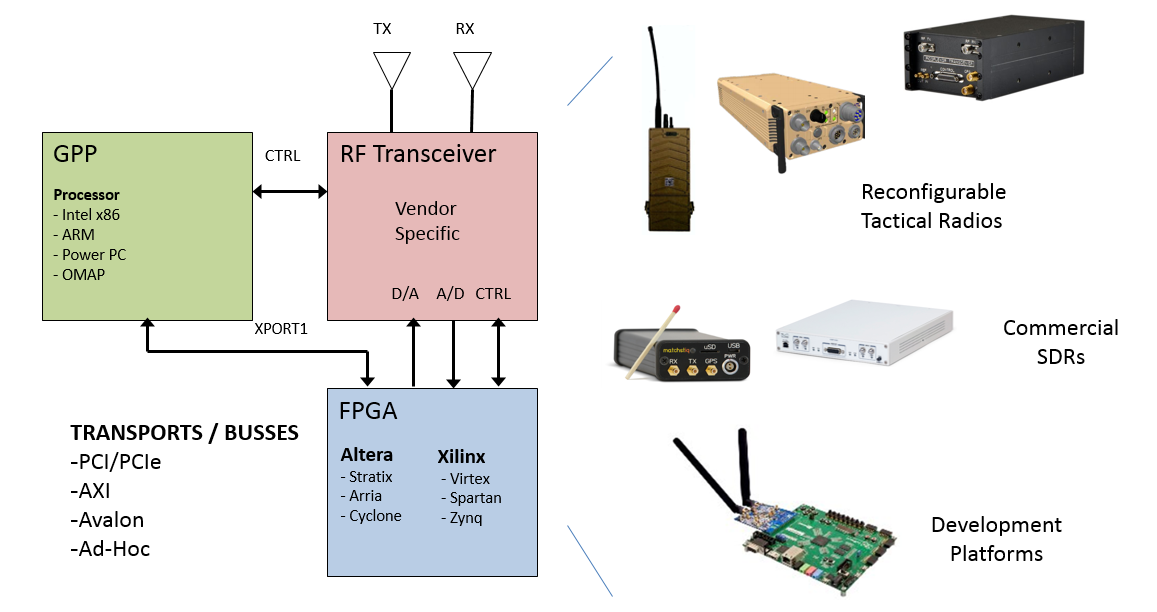
\includegraphics[scale=0.4]{./figures/sdr_block_diagram.png}
        \caption{Block diagram of a typical OpenCPI software-defined radio system (left). Examples systems with this block diagram (right)}
        \label{fig:sdr_block_diagram}
\end{figure}
\newpage
Figure \ref{fig:con_op} illustrates OpenCPI's concept of operation. Components are developed as functions independent of intended application and aggregated into libraries. They are developed for a processor type (GPP, FPGA) using C++ or VHDL using portable coding practices so that they can execute on differing system architectures. The framework's code generators wrap the component and generate standardized interfaces for interconnection with other components.\par
OpenCPI applications are comprised of one or more components and can be a mix of GPP and FPGA functions. The framework build engine generates all the required code to connect the components together and uses the vendor compilers to generate executables for the target system.\par
\begin{figure}[ht]
        \centering
        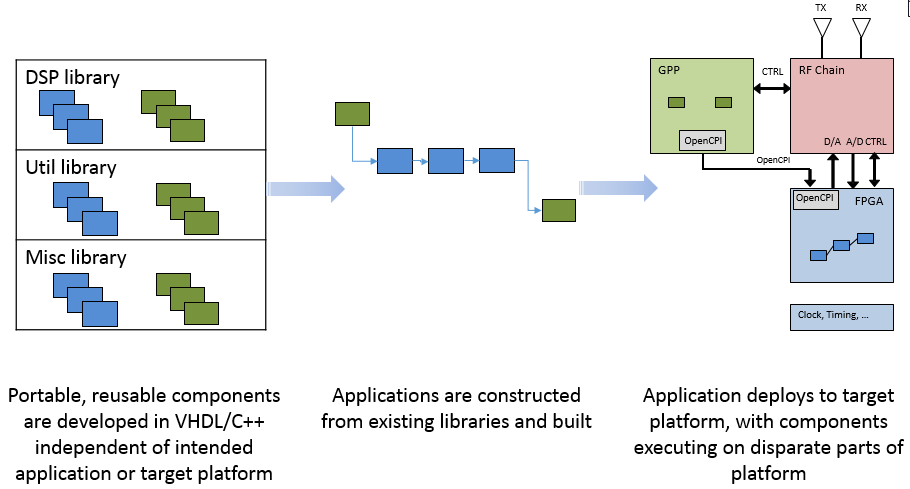
\includegraphics[scale=0.5]{./figures/concept_of_operation.png}
        \caption{OpenCPI concept of operation}
        \label{fig:con_op}
\end{figure}
During application deployment, the OpenCPI runtime platform manages the application from start to finish, including identifying the requirements of the application, detecting available systems, loading component executables to matching processors, setting up control and data pathways, and configuring the RF transceiver.
\section*{What knowledge is needed to use OpenCPI?}
There are three types of OpenCPI development:
\begin{enumerate}
\item Application development
\item Component development
\item Platform development
\end{enumerate}

Application development using existing component libraries only requires knowledge of the OpenCPI framework. Component development involves creating new components and requires knowledge of C++ for software development or VHDL for FPGA development and knowledge of the framework. Platform development is the process of enabling a system to execute OpenCPI applications. It requires both Application and Component development skills as well as more specialized knowledge of system interconnect architecture and OpenCPI framework interfaces.

\section*{What is included with OpenCPI?}
All of the following are included in an OpenCPI release:
\begin{itemize}
\item RPMs for installation
\item Integrated development environment(IDE)
\item Projects with example components and reference applications
\item Documentation including installation guides, user guides, and component data sheets
\end{itemize}

\section*{How can I learn more about OpenCPI?}
There are a number of resources for learning more about the OpenCPI framework. It is recommended to start with the Installation and Introductory Resources, and the other resources can be used depending on skill set and type of development being performed.
\subsubsection*{Installation and Introductory Resources}
\begin{itemize}
\item \textit{Acronyms and Definitions}
\item \textit{Installation Guide}
\item \textit{Getting Started Guide}
\item \textit{OpenCPI Application Development}
\item \textit{OpenCPI Component Development}
\item \textit{IDE Guide}
\end{itemize}
In addition to these documents, there are platform specific Getting Started Guides which can be used to begin developing on existing OpenCPI platforms.
\subsubsection*{FPGA Component Development Resources}
These resources are related specifically to FPGA development in the framework.
\begin{itemize}
\item \textit{FPGA Vendor Tools Installation Guide}
\item \textit{OpenCPI HDL Development}
\end{itemize}
\subsubsection*{GPP Component Development Resources}
These resources are related specifically to GPP development in the framework.
\begin{itemize}
\item \textit{OpenCPI RCC Development}
\end{itemize}
\subsubsection*{Platform Development Resources}
These resources are related specifically to platform development in the framework.
\begin{itemize}
\item \textit{OpenCPI Platform Development}
\end{itemize}
\subsubsection*{Support Resources}
In addition to these documents, there is more specialized documentation included with the OpenCPI release. Please refer to the documentation package for further information. Additionally, questions and further support for the framework can be obtained via email at discuss@lists.opencpi.org.
\subsubsection*{OpenCPI Application and Component Developer Training}
OpenCPI Application and Component Developer Training Materials are available which include labs and lecture slides. The training reviews how to create an OpenCPI project, create GPP components in C++ and FPGA components in VHDL, and how to develop and execute applications on the Epiq Matchstiq Z1 SDR all using the ANGRYVIPER IDE. It is intended to be self-guided, but instructor led training is offered occasionally on request.\par\bigskip
\end{document}
